 \documentclass[11pt,a4paper]{article}
\usepackage[a4paper,margin=2cm]{geometry}
\usepackage[]{graphicx}
\usepackage{bm}
\usepackage[strings]{underscore}
\usepackage{apacite}
\bibliographystyle{apacite}
\usepackage{svg}
\usepackage{amsmath}
\setlength{\parindent}{0pt}
\graphicspath{ {./images} }
\usepackage{wrapfig}
\usepackage{float}
\usepackage[autostyle, english = american]{csquotes}
\usepackage[toc,page]{appendix}
\usepackage{amssymb}
\MakeOuterQuote{"}
\usepackage[T1]{fontenc}
\svgpath{./Diagrams}

\begin{document}

\begin{titlepage}


\title{Determining the relationship between masses in equilibrium and the angle of a frictionless plane}

\author{Noah Alexiou}


\date{May 2025}

\maketitle
\centering

\end{titlepage}
\tableofcontents
\newpage

\section{Introduction}

\subsection{Research Question}
When the mass of an  on a frictionless plane is altered, and the mass of a hanging object adjusted so  equilibrium is achieved, can this be used to measure the angle of the plane? What is the accuracy and uncertainty of this method in comparison to conventional measuring techniques. 

\subsection{Rationale}

The original experiment was conducted to confirm the relationship between the mass of a carriage ($C_m$) and a hanging mass($H_m$) when a frictionless plane was inclined at different angles. In theory $C_m$ should have been 

It was found during the experiment that the angle measurement device, an `angle gun', had a large uncertainty ($\pm1\deg$) compared to the scale used to measure masses ($\pm0.01$). Considering the established relationship between the masses, it was questioned whether the relationship between the masses in equilibrium could be used to determine the angle of the plane with improved accuracy and reduced uncertainty. 
\newline
\newline
Considering Newtons first law, under equilibrium the net force is 0 \cite{encyclopediabritannica_2023_newtons}. If we consider how the data will be plotted once recorded then we can find $\theta$ in terms of $H_m$, and $C_m$. 
\begin{center}
	\begin{align*}
	H_m= &C_m\cdot{\sin(\theta)} \\
	\frac{H_m}{C_m}=&\frac{1}{\mathrm{gradient}}=\sin(\theta)\\
	\therefore \sin^{-1}\left(\frac{H_m}{{C_m}}\right)=&\sin^{-1}\left(\frac{1}{\textrm{gradient}}\right)=\theta
	\end{align*}
\end{center}



Since we now have the angle in terms of the gradient, we can use it to find the uncertainty in the angle. 
This implies the uncertainty in the gradient is equivalent to uncertainty in the angle. 

\includegraphics[width=0.8\paperwidth]{./Diagrams/set_upV2.png}


\subsection{Methodology}

\subsubsection{Modifications}


The following modifications to the method were implemented
\begin{itemize}
	\item The plane was kept at a constant angle throughout the entire duration of the experiment. This was done to isolate it from the independent and dependent variables and ensure that the results of all trials would point to the same relationship between them and the angle.
	\item The independent variable became the hanging mass ($H_m$) to reduce uncertainty in its force via removing factors such as unaccounted for friction and unnecessary trigonometric calculations. This places as much of the uncertainty as possible on the dependent variable, therefore allowing it to be measured more easily.
	\item The dependent variable became the carriage mass ($C_m$) as the large area inside each carriage allowed for fine adjustment of its mass via the addition of brass weights. Multiple carriages could be connected to allow for a greater range of weight's to be added which enhanced this.
\end{itemize}

\subsubsection{Materials}
\begin{itemize}
	\item Angle gun 
	\item Frictionless plane
	\item Brass weights
	\item Blue tack 
	\item Scale
	\item Carriage
\end{itemize}

\subsubsection{Method}
\begin{enumerate}
\item Set up slope at a constant angle. It will remain at this angle for the entire duration of the experiment. 
\item Set the hanging mass ($H_m$) to its minimum value initially.
\item Alter the mass of the carriage $(C_m)$ until equilibrium with the $H_m$ is achieved.
\item Measure and record masses. 
\item Repeat for 3 trials with current $H_m$ value.
\item Increase $H_m$ by 50 grams. 
\item Repeat for each $H_m$ value.
\end{enumerate}


\subsubsection{Risk Assessment}
Frictionless plane
\begin{itemize}
	\item Mishandling of heavy masses on the frictionless plane could result in them sliding down the slope at high speed. This could damage equipment of cause injury. The slope will be turned off not required, and one person will always be supporting the carriage whenever possible to prevent this. 
	\item Using too low fan speed on the frictionless plane may not create enough of an air pocket to support heavy weights. This could cause rubbing between the surfaces which could damage both the plane and carriage. The plane will be set to the highest possible speed throughout the experiment to negate the possibility of this occurring.
\end{itemize}
Masses
\begin{itemize}
	\item Heavy masses or items containing many brass weights may cause injury if dropped or mishandled. participants will wear enclosed footwear to negate injury if this occurs.  
\end{itemize}
\section{Results and Evaluation}
\subsection{Results}

\subsubsection{Raw Data}
\begin{center}
	\centering
	\begin{figure}[h]
		\centering
		\includegraphics[width=0.83\paperwidth]{resultstable.png}
		\caption{Raw results with additional calculations}
	\end{figure}
	
\end{center}


\subsubsection{Sample Calculations}
\begin{center}
\textbf{Absolute uncertainty for $C_m$ when $H_m=50.160$}
\begin{align*}
	\sigma(C_m)=&\pm\frac{\textrm{max}-\textrm{min}}{2}\\
	=&\pm\frac{139.20-138.55}{2}
	\\=&\pm0.33
\end{align*}
\newline


\textbf{Average mass of $C_m$ when $H_m=50.16$}
\begin{align*}
		\bar{C_m}=&\frac{\Sigma^n_{i=1}C_m}{n}\\
		=&\frac{138.55+139.20+138.54}{3}\\
		=&137.76
	\end{align*}
\end{center}

\subsubsection{Plotting}

\begin{figure}[H]
\centering
\includegraphics[width=0.8\paperwidth]{results.png}
\caption{Average $H_m$ and $C_m$ values}
\end{figure}




\section{Discussion}
\subsection{Analysis of evidence}


\subsection{Evaluation}


\section{Conclusion}
\newpage

\bibliography{./Bibliography/Physics_IA2.bib}

	
\end{document}